\documentclass[12pt,letterpaper]{article}
\usepackage{fullpage}
\usepackage[top=2cm, bottom=4.5cm, left=2.5cm, right=2.5cm]{geometry}
\usepackage{amsmath,amsthm,amsfonts,amssymb,amscd}
\usepackage{lastpage}
% \usepackage{hyperref}
\usepackage{enumerate}
\usepackage{fancyhdr}
\usepackage{mathrsfs}
\usepackage{xcolor}
\usepackage{graphicx}
\usepackage{listings}
%\usepackage{mcode}
%\usepackage{hyperref}
\usepackage{movie15}
\usepackage{float}


\usepackage[colorlinks = true,
            linkcolor = blue,
            urlcolor  = blue,
            citecolor = blue,
            anchorcolor = blue]{hyperref}

% load package with ``framed'' and ``numbered'' option.
\usepackage[framed,numbered,autolinebreaks,useliterate]{mcode}

% \hypersetup{%
%   colorlinks=true,
%   linkcolor=blue,
%   linkbordercolor={0 0 1}
% }
 
% \renewcommand\lstlistingname{Algorithm}
% \renewcommand\lstlistlistingname{Algorithms}
% \def\lstlistingautorefname{Alg.}

% \lstdefinestyle{Python}{
%     language        = Python,
%     frame           = lines, 
%     basicstyle      = \footnotesize,
%     keywordstyle    = \color{blue},
%     stringstyle     = \color{green},
%     commentstyle    = \color{red}\ttfamily
% }

\setlength{\parindent}{0.0in}
\setlength{\parskip}{0.05in}

% Edit these as appropriate
\newcommand\course{Digital Signal Processing}
\newcommand\hwnumber{4}                  % <-- homework number
\newcommand\NetIDa{Mehdi Raza Khorasani}           % <-- NetID of person #1
\newcommand\NetIDb{}           % <-- NetID of person #2 (Comment this line out for problem sets)

\pagestyle{fancyplain}
\headheight 35pt
\lhead{\NetIDa}
\lhead{\NetIDa\\\NetIDb}                 % <-- Comment this line out for problem sets (make sure you are person #1)
\chead{\textbf{\Large Homework \hwnumber}}
\rhead{\course \\ \today}
\lfoot{}
\cfoot{}
\rfoot{\small\thepage}
\headsep 1.5em

\begin{document}
\section*{Signal Analysis}
The N point DFT of signal was taken with $N = 2097152$. The Magnitude response is shown in figure \ref{f1}

\begin{figure}[!h]
    \centering
    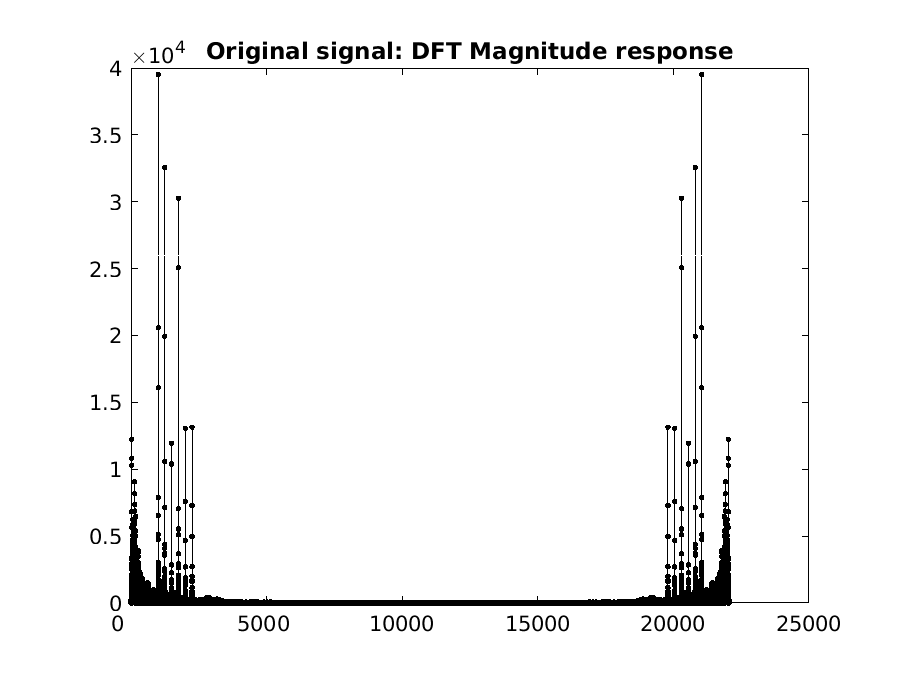
\includegraphics{figure/dft_original.eps}
    \caption{DFT of original signal}
    \label{f1}
\end{figure}

\section*{Filter Design}
We know that our ears are indifferent to phase shifts, so an IIR filter can be used for efficiency. Using MATLAB DSP system toolbox's filter designer, we select a band stop filter with the following Frequency characteristics: 
\begin{enumerate}
    \item $F_{pass1} = 1920 Hz$
    \item $F_{stop1} = 1990 Hz$
    \item $F_{stop2} = 5000 Hz$
    \item $F_{pass2} = 5500 Hz$
    \item Design Method: IIR Elliptic
    \item Order = 18
\end{enumerate}
The order 
The magnitude response and PZ plot of the filter is given in figure \ref{f2} and \ref{f3} respectively. 

\begin{figure}[!h]
    \centering
    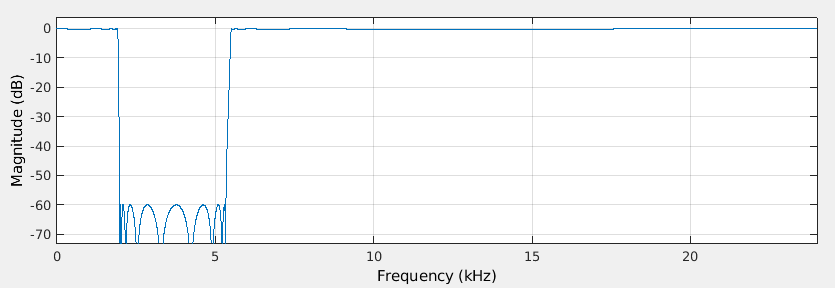
\includegraphics[scale = 0.5]{figure/filter_res1.png}
    \caption{Filter Magnitude response}
    \label{f2}
\end{figure}
\begin{figure}[!h]
    \centering
    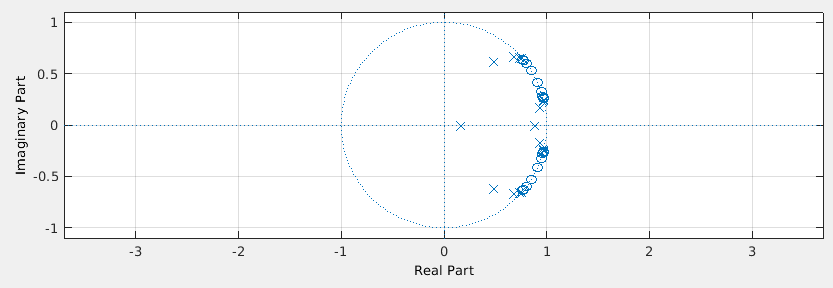
\includegraphics[scale = 0.5]{figure/filter_pz.png}
    \caption{Filter PZ plot}
    \label{f3}
\end{figure}

\section*{Filtered Signal}
Passing the signal through the above designed filter, we get the resulting signal's frequency response as shown in figure \ref{f4}.

\begin{figure}[!h]
    \centering
    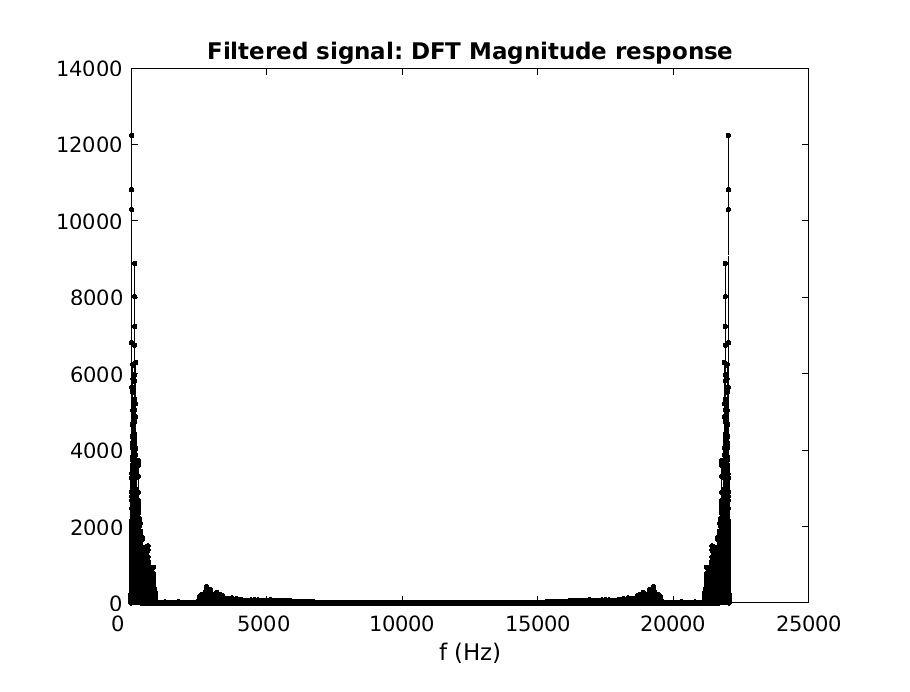
\includegraphics{figure/dft_filtered.eps}
    \caption{Filtered magnitude response}
    \label{f4}
\end{figure}

If we play back the filtered .wav (attached), it can observed that all noises have been eliminated.  

\section*{MATLAB codes}
The following script was used: 

\begin{lstlisting}
%% reading File: 
Fs = 44100; 
[s,Fs]=audioread('NoisyHUAnthem.wav'); 
% sound(s,Fs); 
pause(5); 

%% Analysis: 
N = length(s); % determine length of signal 
n = ceil(log2(N)); % ceil to the closest power of 2
N = 2^n; % use this N for fft 
X= fft(s, N); 

f = linspace(0, Fs,N);
stem(f, abs(X), '.')

set(gca, 'XTickLabel', get(gca, 'XTick'));
title('Original signal: DFT Magnitude response')
print -deps dft_original.eps

%% Filtering: 
close all
filter_coeffs = load('lpf_a.mat')
filtered = filter(filter_coeffs.Hd, s);
sound(filtered,Fs);

%calculate fft: 
N = length(filtered); % determine length of signal 
n = ceil(log2(N)); % ceil to the closest power of 2
N = 2^n; % use this N for fft 
X= fft(filtered, N);

figure()
stem(f, abs(X), '.')
title('Filtered signal DFT')
xlabel('f (Hz)')
set(gca, 'XTickLabel', get(gca, 'XTick'));
title('Filtered signal: DFT Magnitude response')
print -deps dft_filtered.eps
audiowrite('recovered.wav', filtered, Fs)

\end{lstlisting}
\end{document}
